%%%%%%%%%%%%%%%%%%%%%%%% 
% Dokumentinformationen %
%%%%%%%%%%%%%%%%%%%%%%%%%
\documentclass{scrartcl}

\include{header/zusammenfassung}

\title{TSM\_AdvContr}
\subtitle{Advanced Control}
\author{L.~Schmid, H.~Diethelm, H.~Badertscher}


\usepackage{wrapfig}
\newcommand{\matlab}[1]{\footnotesize{(Matlab: \texttt{#1})}\normalsize{}}
\newenvironment{aufzaehlung}[0]{
    \begin{enumerate}\setlength{\leftmargin=0.5cm \itemsep}{1pt}\setlength{\parskip}{0pt}\setlength{\parsep}{0pt}}
  {\end{enumerate}}      
\DeclareMathOperator{\rank}{rank}

\let\Re\relax
\DeclareMathOperator{\Re}{Re}

%TODO: english!
%TODO: no script-size!

\begin{document}

    \section{Zustandsraumdarstellung}
\scriptsize
Darstellung einer Differentialgleichung $n$. Ordnung durch ein
Differentialgleichungssystem von $n$ Gleichungen 1. Ordnung.

\subsection{Definition}
\begin{tabular}{ll}
\parbox{10cm}{
	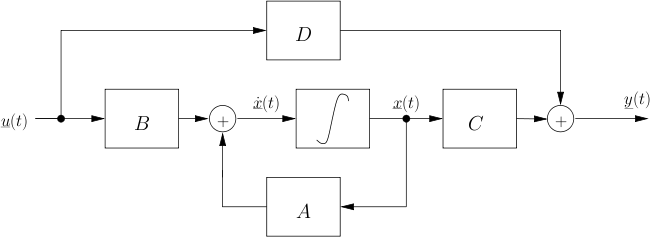
\includegraphics[width=10cm]{./bilder/zrd-schema.png}
	}
	& \parbox{8cm}{
		$\dot{\underline{x}}(t) = {\boldsymbol A} \underline{x}(t) + {\boldsymbol B}
		\underline{u}(t)$ \\
		$\underline{y}(t) = {\boldsymbol C} \underline{x}(t) + {\boldsymbol D}
		\underline{u}(t)$\\ 
		
		${\boldsymbol A}$: Systemmatrix ($n$ x $n$): Spalten entsprechen Ausgängen
		der Integratoren, Zeilen Eingänge ; \\ 
		${\boldsymbol B}$: Steuer- oder
		Eingangsmatrix ($n$ x $m$) ``senkrecht''; \\ ${\boldsymbol C}$: Beobachtungs- oder Ausgangsmatrix ($k$ x $n$)
		``waagrecht''; \\
		${\boldsymbol D}$: Übergangs- oder Durchgangsmatrix ($k$ x
		$m$)\\
		
		wobei $m$ der Anzahl Eingangssignale, $k$ der Anzahl Ausgangssignale \& $n$ der
		Anzahl Zustandsgrössen (Integratoren, Ordnung) entsprechen.\\
	}
 \end{tabular}


\subsection{ZRD im Frequenzbereich \matlab{ss2tf}}
$$\boldsymbol{G(s)} = \frac{\underline{Y}(s)}{\underline{U}(s)} =
\boldsymbol{C}\left(s\boldsymbol{I_n}-\boldsymbol{A}\right)^{-1}\boldsymbol{B}+\boldsymbol{D}$$
\\
Die Grösse der Matrix $\boldsymbol {G(s)}$ entspricht der Grösse der
Durchgangsmatrix $\boldsymbol D$. $\boldsymbol{I_n}$ sei die Einheitsmatrix mit
Grösse $n$ x $n$.

\subsection{Übertragungsmatrizen}
$$G(s)=\frac{Y(s)}{U(s)}=\frac{b_{m} s^{m} + b_{m-1} s^{m-1} +\cdots+b_{1} s 
+ b_{0}}{s^{n} + a_{n-1} s^{n-1} + \cdots + a_{1} s + a_{0}}$$\\
Allgemeine Formel für $m=1$ Eingang, $k=1$ Ausgang, $n=2$ Integratoren:\\
$$G(s) = \left [ 
\begin{array}{c c}
C_{11}  & C_{12}\\
\end{array}
\right ]\cdot
\left (
\left [ 
\begin{array}{cc}
 s & 0\\
0 & s\\
\end{array}
\right ] -
\left [ 
\begin{array}{cc}
 A_{11} & A_{12}\\
 A_{21} & A_{22}\\
\end{array}
\right ]
\right )^{-1}\cdot
\left [ 
\begin{array}{c}
 B_{11}\\
 B_{21}\\
\end{array}
\right ]+ D$$
$$=  \frac{B_{11}C_{11}(s-A_{22}) + B_{11}C_{12}A_{21} +
B_{21}C_{11}A_{12} + B_{21}C_{12}(s-A_{11})}{(s-A_{22})(s-A_{11}) - A_{12}A_{21}} + D$$


\subsection{Stabilität}
Wenn alle Realteile der Eigenwerte $\lambda$ der Systemmatrix ${\boldsymbol A}$
negativ sind, ist ein LTI-System asymptotisch stabil, jedoch nicht umgekehrt:
$\left | \lambda\boldsymbol{I} - \boldsymbol{A} \right |   =0 \rightarrow \forall~\lambda \quad\Re \{\lambda\}<0$

\subsection{Beobachtbar- \& Steuerbarkeit}
\subsubsection{Steuerbarkeit \matlab{ctrb}}
Gibt es Zustände von $\underline{x} (t)$ die nicht von den
Eingängen $\underline{u} (t)$ beeinflusst werden? Wenn ja,
dann ist das System nicht steuerbar!

Wenn $rank \left[P_{c}\right] = rank \left[ \boldsymbol{B~~AB~~ A^2B~\ldots~
A^{n-1}B} \right] = n $, dann ist das System vollständig steuerbar.


\subsubsection{Beobachtbarkeit \matlab{obsv}}
Gibt es Zustände $\underline{x}(t)$ die keinen Einfluss auf die Ausgänge
$\underline{y}(t)$ haben? Wenn ja, kann man aus dem Verhalten von 
$\underline{y}(t)$ nicht auf die Zustände $\underline{x}(t)$ schliessen!
Das System ist nicht beobachtbar!


Wenn $rank \left[P_{o}\right] = rank \left[ \boldsymbol{
\begin{array}{c}
 C\\
 CA\\
CA^2\\
\vdots \\
CA^{n-1}\\
\end{array}} \right] = n$, dann ist das System vollständig
beobachtbar.

\subsubsection{Regelungsnormalform}
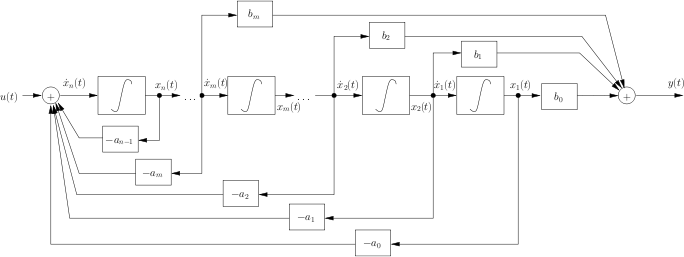
\includegraphics[width=10cm]{./bilder/zrd-regelungsnormalform.png} \\
\scriptsize
$$G(s)=\frac{Y(s)}{U(s)}=\frac{b_{n-1} s^{n-1} + b_{n-2} s^{n-2} +\cdots+b_{1} s 
+ b_{0}}{s^{n} + a_{n-1} s^{n-1} + \cdots + a_{1} s + a_{0}} + d$$\\
\begin{eqnarray*}
\left [ 
\begin{array}{c}
\dot{x}_1(t)\\
\dot{x}_2(t)\\
\vdots\\
\dot{x}_{n-1}(t)\\
\dot{x}_{n}(t)\\
\end{array}
\right ] &=&
\left [ 
\begin{array}{c c c c c}
0 & 1 & 0 & \ldots & 0\\
0 & 0 & 1 & \ldots & 0\\
\vdots & \vdots & \vdots & \ddots & \vdots\\
0 & 0 & 0 & \ldots & 1\\
-a_0 & -a_1 & -a_2 & \ldots & -a_{n-1}\\
\end{array}
\right ]\cdot
\left [ 
\begin{array}{c}
x_1(t)\\
x_2(t)\\
\vdots \\
x_{n-1}(t)\\
x_{n}(t)\\
\end{array}
\right ]+
\left [ 
\begin{array}{c}
0 \\
0\\
\vdots\\
0\\
1\\
\end{array}
\right ]\cdot
u(t),\\
y(t) &= &
\left [ 
\begin{array}{c c c c}
b_0 & b_1 & \ldots & b_{n-1}\\
\end{array}
\right ] \cdot
\left [ 
\begin{array}{c}
x_1(t)\\
x_2(t)\\
\vdots \\
x_{n-1}(t)\\
x_{n}(t)\\
\end{array}
\right ]+
\left [ 
\begin{array}{c}
d \\
\end{array}
\right ] \cdot
u(t).
\end{eqnarray*}
\normalsize


\subsubsection{Beobachtungsnormalform}
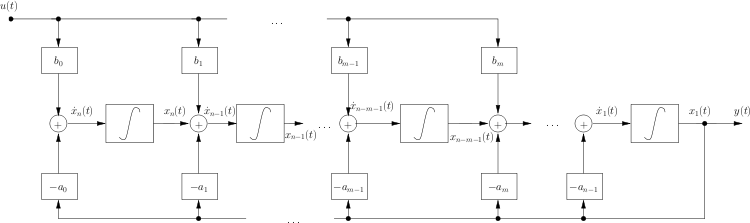
\includegraphics[width=10cm]{./bilder/zrd-beobachtungsnormalform.png} \\
\scriptsize
$$G(s)=\frac{Y(s)}{U(s)}=\frac{b_{n-1} s^{n-1} + b_{n-2} s^{n-2} +\cdots+b_{1} s 
+ b_{0}}{s^{n} + a_{n-1} s^{n-1} + \cdots + a_{1} s + a_{0}} + d$$\\
\begin{eqnarray*}
\left [ 
\begin{array}{c}
\dot{x}_1(t)\\
\dot{x}_2(t)\\
\vdots\\
\dot{x}_{n-1}(t)\\
\dot{x}_n(t)\\
\end{array}
\right ] &=&
\left [ 
\begin{array}{c c c c c}
0 & 0 & 0 & \ldots & -a_0\\
1 & 0 & 0 & \ldots & -a_1\\
0 & 1 & 0 & \ldots & -a_2\\
\vdots & \vdots &  \ddots & 0 & \vdots\\
0 & 0 & \ldots & 1 & -a_{n-1}\\

\end{array}
\right ]\cdot
\left [ 
\begin{array}{c}
x_1(t)\\
x_2(t)\\
\vdots \\
x_{n-1}(t)\\
x_{n}(t)\\
\end{array}
\right ]+
\left [ 
\begin{array}{c}
b_0 \\
b_1\\
b_2\\
\vdots\\
b_{n-1}\\
\end{array}
\right ]\cdot
u(t),\\
y(t) &= &
\left [ 
\begin{array}{c c c c}
0 & 0 & \ldots & 1\\
\end{array}
\right ] \cdot
\left [ 
\begin{array}{c}
x_1(t)\\
x_2(t)\\
\vdots \\
x_{n-1}(t)\\
x_{n}(t)\\
\end{array}
\right ]+
\left [ 
\begin{array}{c}
d \\
\end{array}
\right ] \cdot
u(t).
\end{eqnarray*}
\normalsize

    \newpage
    \section{Zustands-Regler}
\subsection{State Feadback}

$A_g = A-BK \; , \; B_g = BK_{vf} \; , \; C_g = C $\\
$G(s) = \frac{\underline{Y}(s)}{\underline{U}(s)} = C(sI-A+BK)^{-1}BK_{vf}$\\
$K_{vf} = (C(-A+BK)^{-1}B)^{-1}$

\subsection{Pole Placement}

\begin{tabular}{ll}
	\parbox{8cm}{$det(\lambda I-A+BK) = (\lambda - \lambda_1)...(\lambda - \lambda_n)$} &
	\parbox{3cm}{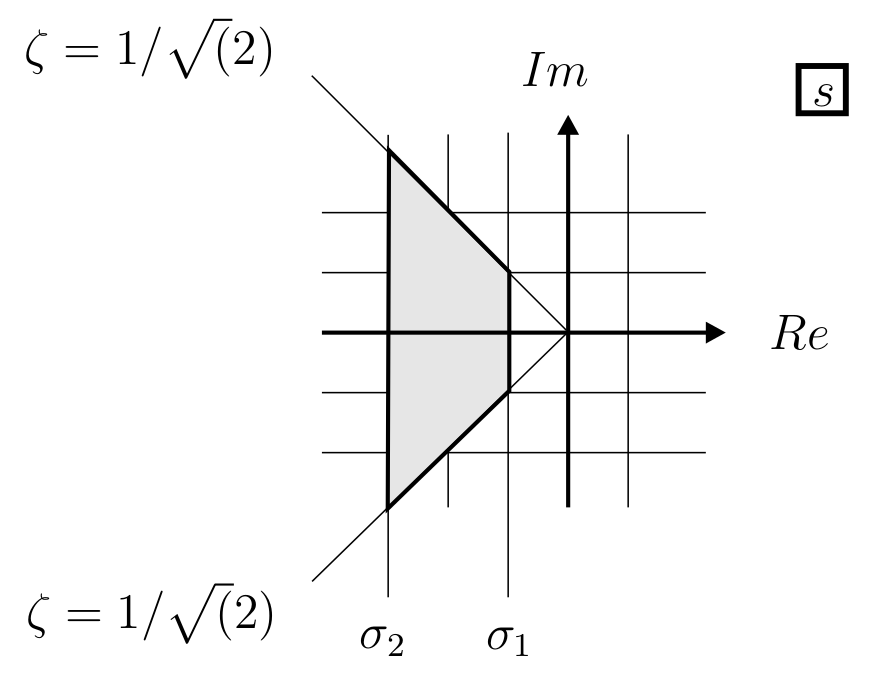
\includegraphics[width=3cm]{./bilder/pole_locations.png}}
\end{tabular}

\subsection{Series Connection}
System 1:
$x_1' = A_1x_1 + B_1u$ \quad
$y_1 = C_1x_1 + D_1u$ \qquad
System 2: 
$x_2' = A_2x_2 + B_2y_1$ \quad
$y_2 = C_2x_2 + D_2y_1$

\begin{tabbing}
State equation \quad \=
$\begin{bmatrix}x_1' \\ x_2'\end{bmatrix} 
     = \begin{bmatrix}
       A_1 & 0 \\ 
       B_2C_1 & A_2
     \end{bmatrix} 
     \begin{bmatrix}
       x_1 \\ 
       x_2
     \end{bmatrix} +
     \begin{bmatrix}
       B_1 \\ 
       B_2D_1
     \end{bmatrix}u$\\
       
Output equation \>
$\begin{bmatrix}y_2 \\ y_1\end{bmatrix} 
     = \begin{bmatrix}
      C_1 & 0 \\ 
      D_2C_1 & C_2
     \end{bmatrix} 
     \begin{bmatrix}
       x_1 \\ 
       x_2
     \end{bmatrix} +
     \begin{bmatrix}
       D_1 \\ 
       D_2D_1
     \end{bmatrix}u$
\end{tabbing}


\newpage

\subsection{LQR-Entwurf (Linear-quadratic regulator)}
	\begin{tabular}{ll}
		\parbox{6cm}{	$J(K_R,T_N,\ldots)=\int\limits^{\infty}_0 e(t)^2 dt = minimal$\\
						$J=\int\limits_0^{\infty} {x^T Q x+u^T R u}= minimal$\\}&
		\parbox{6cm}{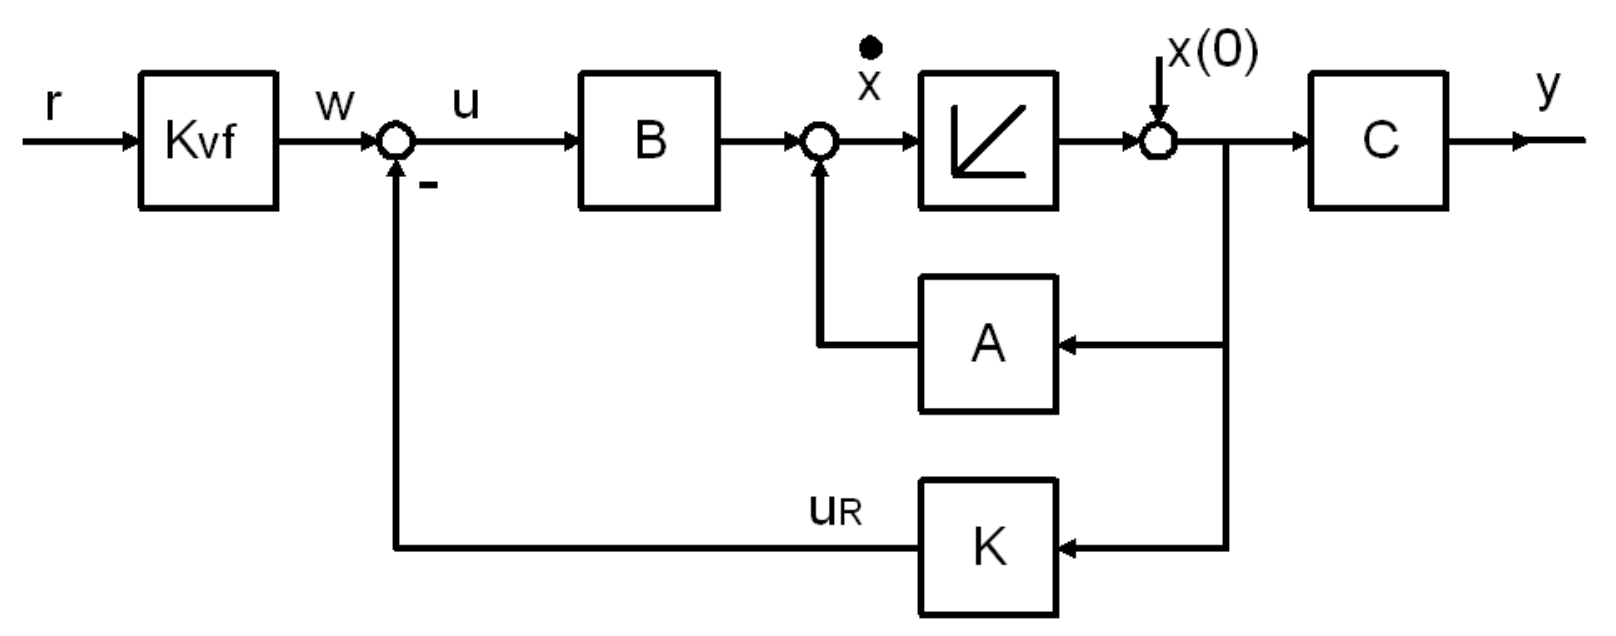
\includegraphics[width=6cm]{./bilder/statereg.png}}
	\end{tabular}\\	
	Q,R: positive definite; Bei SISO ist R eine Zahl\\
	Optimum: Riccati equation\\
	$ A^T P + P A - P B R^{-1} B^T P = -Q$ \hspace{2cm}
	P ist die L"osungsmatrix
	\begin{aufzaehlung}
    	\item $\dot{x} = Ax + Bu \; / \;  Q \; \text{und} \; R \; \text{gegeben}$
    	\textbf{meist} wird f"ur Q=I und R=1 eingesetzt.
    	\item L"osungsmatrix P bestimmen (aus der L"osungsmenge den positiv
    	definierten Wert)
    	\item Reglervektor berechnen $K=R^{-1} B^T P$
    \end{aufzaehlung}

\subsection{LQG-Entwurf (Linear-quadratic gaussian / Observer)}
	\begin{tabular}{ll}
		\parbox{12cm}{	Duale Korrespondenzen:\\
						\begin{eqnarray*}
						\textbf{LQR} &\Leftrightarrow& \textbf{LQG} \\
						P_c &\Leftrightarrow& P_o^T\\
						B &\Leftrightarrow& C^T\\
						A &\Leftrightarrow& A^T\\
						K &\Leftrightarrow& H^T\\
						A - BK &\Leftrightarrow& A - HC\\
						det(\lambda I-A+BK) &\Leftrightarrow& det(\lambda I-A+HC) \\
						A^T P + P A - P B R^{-1} B^T P = -Q &\Leftrightarrow& A P + P A^T - P C^T R^{-1} C P = -Q \\
						K=R^{-1} B^T P &\Leftrightarrow& H=(R^{-1} CP)^T = PC^TR^{-1}
						\end{eqnarray*}
					}
		\parbox{6cm}{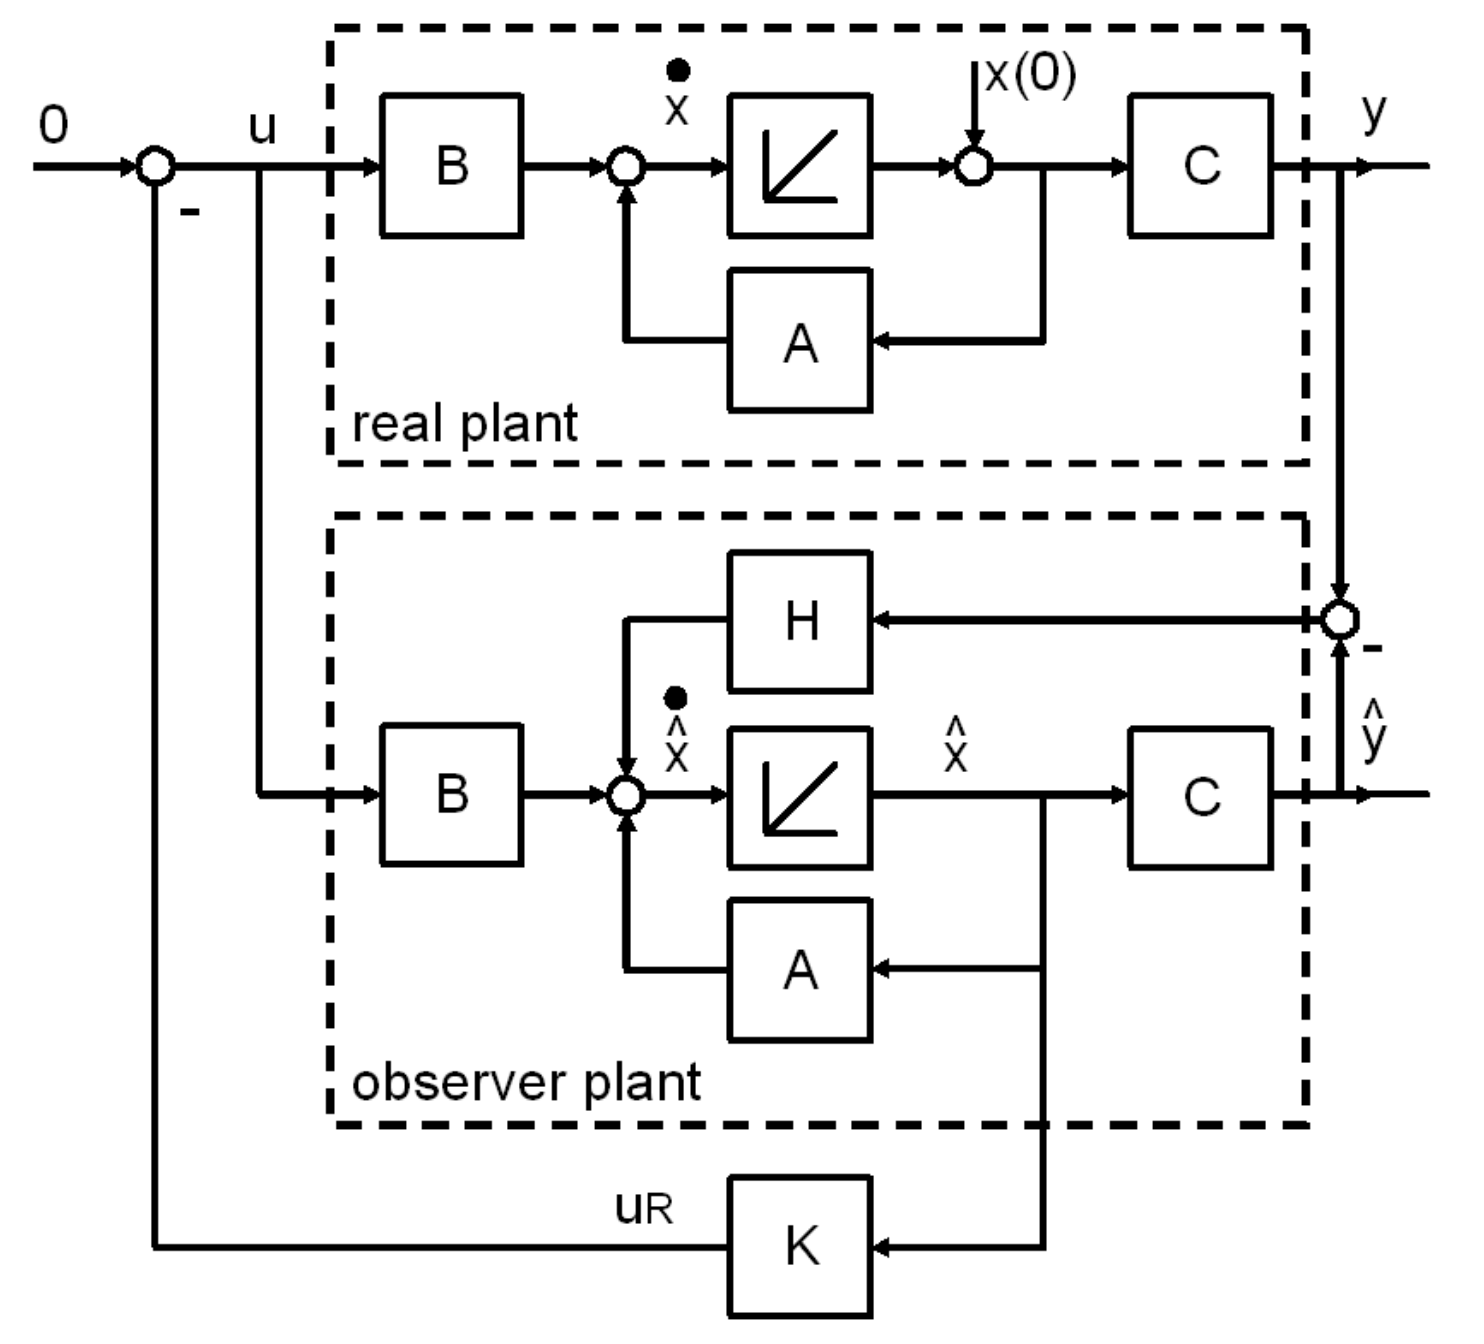
\includegraphics[width=6cm]{./bilder/observer.png}}
	\end{tabular}\\
	
\subsection{LQR/LQG Entwurf}
\begin{tabular}{ll}
	\parbox{6cm}{Gesamtsystem: \\ $
			\begin{bmatrix}
				\dot{x}\\
				\dot{\tilde{x}}\\
			\end{bmatrix} = 
			\begin{bmatrix}
				A-BK && BK\\
				0 && A-HC\\
			\end{bmatrix} 
			\begin{bmatrix}
				x\\
				\tilde{x}\\
			\end{bmatrix}
			$} &
	\parbox{6cm}{Charakteristik:\\ $
			det 
			\begin{bmatrix}
				sI - A + BK && -BK\\
				0 && sI - A + HC\\
			\end{bmatrix}=$\\
			$det(sI-A+BK)*det(sI-A+HC)=0$}
\end{tabular}
	
\subsection{LQR/LTR und LQR/LTR Entwurf}

\begin{tabular}{ll}
	\parbox{8cm}{
		LQR/LTR
		\begin{itemize}
			\item LQR beliebige Gewichtung
			\item LQG mit $Q=\rho BB^T \; / \; R=I  \; / \; \rho > 0$
		\end{itemize}}
	\parbox{8cm}{
			LQG/LTR
			\begin{itemize}
				\item LQR mit $Q=\rho C^TC \; / \; R=I  \; / \; \rho > 0$
				\item LQG beliebige Gewichtung
			\end{itemize}}
\end{tabular}		

    
    \newpage
    \section{System Identification}
%TODO: add example for ARX with least squares

\subsection{Nonparametric Identification}

\subsubsection{One Frequency at a Time}
\begin{minipage}{10cm}
Given an LTI system with a transfer function $G_c(s)$ a sinusoidal 
input signal $u(t) = A \cdot \sin(\omega_0 t)$ will create a sinusoidal
signal $y(t) = B \cdot \sin(\omega_0 t + \varphi) + \text{transient terms}$.
The gain $K = B/A$ can be measured at various frequencies to determine
$G_c(j\omega)$ point-wise.
\end{minipage}
\hspace{0.5cm}
\begin{minipage}{8cm}
    \centering
    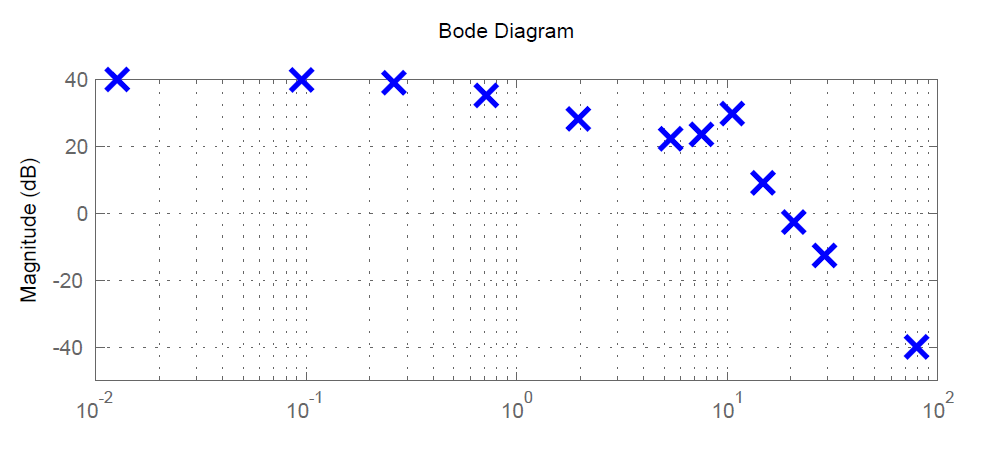
\includegraphics[width=8cm]{bilder/ident_bode.png}
\end{minipage}

\paragraph{Discrete-Time Case}
If the signals $u$ and $y$ are sampled at times $t = kT$, an input
$u(kT) = A \cdot \sin(\omega_0 k T)$
will create the expected output signal
\[
    \hat{y}(kT) = B \cdot \sin(\omega_0 k T + \varphi) 
    = B_c \cdot \cos(\omega_0 k T) + B_s \cdot \sin(\omega_0 k T)
\]
where $B = \sqrt{B_c^2 + B_s^2}$ and $\varphi = \arctan\frac{B_c}{B_s}$.
The sample time $T$ and the number of samples $N$ are chosen to be $T \cdot N = \frac{2\pi}{\omega_0}$.
Then the $B_c$ and $B_s$ which minimize the quadratic cost function reduce to
\begin{align*}
    B_c &= \frac{2}{N}\sum_{k=0}^{N-1} y(kT) \cos(2\pi lk/N) &
    B_s &= \frac{2}{N}\sum_{k=0}^{N-1} y(kT) \sin(2\pi lk/N)
\end{align*}
from which the values $B$ and $\varphi$ can be calculated.
This results in one point of the frequency response $B/A \cdot e^{j\varphi}$.

\subsubsection{Several Frequencies at Once}
The formulas for $B_c$ and $B_s$ are similar to the DFT, which is given by
\[
    \operatorname{DFT}\{f(kT)\} = F_n = \sum_{k=0}^{N-1} f(kT) e^{-j2\pi nk/N}
\]
where $F_n = F(\frac{2\pi n}{NT})$ is the frequency component at the frequency $\omega = \frac{2\pi n}{NT}$.
Using e.g. white noise or chirp signals as input signal $u$, one can calculate the frequency response by
\[
    G_d(e^{j\omega_0 T}) = \frac{\operatorname{DFT}\{y(kT)\}}{\operatorname{DFT}\{u(kT)\}} = \frac{B_s + jB_c}{A}
\]

\subsubsection{Further Nonparametric Methods}

\paragraph{Impulse Response} A discrete-time impulse at the input leads to:
\begin{align*}
    u(kT) &= \begin{cases}
        A & k=0 \\ 0 & k \neq 0
    \end{cases}
    & \Rightarrow &&
    y(kT) &= A \cdot g_d(kT) + v(kT)
\end{align*}
where $v$ is a disturbance and $g_d(kT)$ is the discrete impulse response of the system.

\paragraph{Step Response} A discrete-time step at the input leads to:
\begin{align*}
    u(kT) &= \begin{cases}
        A & k \geq 0 \\ 0 & k < 0
    \end{cases}
    & \Rightarrow &&
    y(kT) &= A \cdot \sum_{m=0}^{k} g_d(mT) + v(kT)
\end{align*}
which allows the estimation of $\hat{g}_d(kT) = \frac{y(kT) - y((k-1)T)}{A}$.

\paragraph{Deconvolution of Output} The output is a convolution of the input $u$ with the
impulse response $g_d$, i.e.
\begin{align*}
    y(0) &= g_d(0) u(0) &
    y(T) &= g_d(0) u(T) + g_d(T) u_0) &
    y(2T) &= g_d(0)u(2T) + g_d(T)u(T) + g_d(2T)u(0) &
    \dots
\end{align*}
If no disturbance $v$ is present, this can be recursively solved for $g_d$ by
\begin{align*}
    \hat{g}_d(0) &= \frac{y(0)}{u(0)} &
    \hat{g}_d(T) &= \frac{y(T) - \hat{g}_d(0)u(T)}{u(0)} = \frac{y(T)u(0) - y(0)u(T)}{u(0)^2} &
    \dots
\end{align*}

\paragraph{Effects of Nonlinearities}
These techniques are \emph{only} applicable to LTI systems.

\subsection{Parametric Identification}
A general model for SISO systems with disturbance $e(k)$ is given by
\[
    A(q) \cdot y(k) = \frac{B(q)}{F(q)} \cdot u(k) + \frac{C(q)}{D(q)}\cdot e(k)
\]
Some often used special cases are:
\begin{align*}
    A(q) \cdot y(k) &= B(q) \cdot u(k) + e(k) & \text{ARX, autoregressive} \\
    A(q) \cdot y(k) &= B(q) \cdot u(k) + C(q) \cdot e(k) & \text{ARMAX, autoregressive moving average} \\
    y(k) &= \frac{B(q)}{F(q)} \cdot u(k) + \frac{C(q)}{D(q)} \cdot e(k) & \text{BJ, Box-Jenkins} \\
    y(k) &= \frac{B(q)}{F(q)} \cdot u(k) + e(k) & \text{OE, output error}
\end{align*}

\subsection{Identifiability}
As example, consider an electromechanical system which is given by
\[
    G(s) = \frac{\frac{K_P K_{\mu} f \Phi}{R J_{\alpha} J_{\beta}}}
    {s^3 + \frac{\Phi^2}{R J_{\alpha}} s^2 + \frac{f(J_{\alpha}+J_{\beta})}{J_{\alpha}+J_{\beta}}s + \frac{f \Phi^2}{R J_{\alpha} J_{\beta}}}
    =
    \frac{b_0}{s^3 + a_2 \cdot s^2 + a_1 \cdot s + a_0}
\]
While the parameter vector $\theta_1 = [a_0 \; a_1 \; a_2 \; b_0]^T$
is \emph{identifiable}, the parameter vector
$\theta_2 = [f \; J_{\alpha} \; J_{\beta} \; \Phi \; R \; K_P \; K_{\mu}]^T$
is \emph{not}, as the model only has five independent matrix entires.
Additional knowledge, e.g. from a datasheet is needed.

\subsubsection{Basics of Least Squares (LS)}
Least squares minimizes the sum of squared errors.
It is used if equations are linear in the parameters $\theta_i$ (l.i.p.).
A form $y = f(u) = \sum_i \theta_i \cdot f_i(u)$ is l.i.p. even if the functions
$f_i(u)$ are nonlinear.

A system of linear equations $y = \Phi \theta$ is solved for $\theta$ by 
$\theta = \Phi^{-1} y$.
If the system is overdetermined, the least squares solution is
\[
    \theta = (\Phi^T \Phi)^{-1} \Phi^T y
\]

\subsubsection{Weighted Least Squares}
Introducing a weighting matrix $L$, the problem becomes $L y = L \Phi \theta$
with the solution
\[
    \theta = (\Phi^T L^T L \Phi)^{-1} \Phi^T L^T L y
\]

\paragraph{Markov Estimation by using the Covariance Matrix}
If the error term $\varepsilon$ has zero mean ($E[\varepsilon]=0$) and the
covariance matrix $V = E[\varepsilon\varepsilon^T]$ and is assumed to be
Gaussian, the optimal estimation for $\theta$ is achieved by using
$L^T L = V^{-1}$.

\subsubsection{Recursive Least Squares}
For large data collections or time-variant processes, the use of recursive methods is of interest.

Given information at time $N$,
\begin{align*}
    \theta_N &= \underbrace{(\Phi_N^T \Phi_N)^{-1}}_{P_N} \Phi_N^T y_N &
    \Phi_N &= \begin{bmatrix} \varphi_0^T \\ \vdots \\ \varphi_N^T \end{bmatrix} &
    y_N &= \begin{bmatrix} y(0) \\ \vdots \\ y(N) \end{bmatrix}
\end{align*}
with
\[
    \varphi_k^T = \begin{bmatrix}
    -y(k-1) & \dots & -y(k-n) & u(k-1) & \dots & u(k-m)
    \end{bmatrix}
\]
the new values at time $N+1$ are found by the recursive formulas
\begin{align*}
    \theta_{N+1} &= \theta_N + \frac{P_N \varphi_{N+1}}{1 + \varphi_{N+1}^T P_N \varphi_{N+1}}\left( y(N+1) - \varphi_N^T \theta_N \right) \\
    P_{N+1} &= P_N - \frac{P_N \varphi_{N+1} \varphi_{N+1}^T P_N}{1 + \varphi_{N+1}^T P_N \varphi_{N+1}}
\end{align*}

\paragraph{Forgetting Factor}
In a slowly time-variant system, old measurements should be forgotten gradually. 
This is achieved by using a \emph{forgetting factor} $\lambda\in]0,1]$ 
(typical values: $0.9 < \lambda < 0.98$) and
\[
    V^{-1} = L^T L = \begin{bmatrix}
        \lambda^N & 0 &\dots & 0 \\
        0 & \ddots & \ddots & \vdots \\
        \vdots & \ddots & \lambda & 0 \\
        0 & \dots & 0 & 1
    \end{bmatrix}
\]
Which leads to the recursive formulas
\begin{align*}
    \theta_{N+1} &= \theta_N + \frac{P_N \varphi_{N+1}}{\lambda + \varphi_{N+1}^T P_N \varphi_{N+1}}\left( y(N+1) - \varphi_N^T \theta_N \right) \\
    P_{N+1} &= \frac{1}{\lambda} \cdot \left(P_N - \frac{P_N \varphi_{N+1} \varphi_{N+1}^T P_N}{\lambda + \varphi_{N+1}^T P_N \varphi_{N+1}}\right)
\end{align*}

\subsection{Practical Aspects of Identification}

\paragraph{Identificatoin Cycle}The identification process is an iterative task.
\paragraph{Sampling Time}An anti-aliasing filter $G_{f}$ must be applied to the analog signal.
\paragraph{Identification of Closed-Loop Systems} A plant might be unstable or
in use for production, or it might contain some built-in feedback mechanisms.
Then the plant has to be identified in a closed loop.
    
    \newpage
    \section{Sampling and extrapolation of signals}

%TODO: well... everything
    %TODO: discrete-time controllers: stability
%TODO: add digital implementation

% % % % % % % % % % % % % % % % % % % %
\section{Discrete-time Plant Models}

\subsection{ZOH-discretization of plant models}
Starting from a continuous-time state-space model $(A,B,C,D)$, the ZOH-discretization is derived.
In continuous-time,
\[
    x(t) = \Phi(t) \cdot x(0) + \Gamma(t) \cdot u(0)
\]
where
\begin{align*}
    \Phi(t) &= \mathcal{L}^{-1} \left( (sI-A)^{-1} \right) = e^{At} &
    & \text{and} &
    \Gamma(t) = \int_0^t \phi(t) \cdot B \cdot dt = \mathcal{L}^{-1} \left((sI-A)^{-1} \cdot B \cdot \frac{1}{s}\right)
\end{align*}

For any sampling time instant, the discrete-time state-space representation is
\begin{align*}
    x_{k+1} &= \Phi(T_s) \cdot x_k + \Gamma(T_s) \cdot u_k \\
    y_k &= C \cdot x_k + D \cdot u_k
\end{align*}

\subsection{ZOH-discretization of transfer functions}
Given a plant model $P(s)$, the ZOH-discretization is
\[
    P_{ZOH}(z) = \frac{z-1}{z}\mathcal{Z}_s\left\{ \frac{P(s)}{s} \right\}
\]

% % % % % % % % % % % % % % % % % % % %
\section{Modelling of discrete-time systems}
A discrete transfer function is gien by
\[
    \frac{Y(z)}{U(z)} = \frac{b_n + b_{n-1}z^{-1}+ \dots + b_0z^{-n}}{1 + a_{n-1}z^{-1} + \dots + a_0}
\]

A discrete-time state-space representation is a matrix difference equation:
\begin{align*}
    x_{k+1} &= F \cdot x_k + G \cdot u_k \\
    y_k &= H \cdot x_k + J \cdot u_k
\end{align*}
which can be written in a transfer function form given by
\[
    P_{ZOH}(z) = H \cdot (zI - F)^{-1} \cdot G + J
\]

\subsection{Properties of sampled systems}

\paragraph{Causality}A transfer function with a higher degree of the numerator is \emph{noncausal}
and is not realizable.

\paragraph{Stability}The stability can be determined using the relation $z = e^{sT_s}$.
The left-half plane in the $s$-domain corresponds to the area inside the unit circle in the $z$-domain.

\paragraph{Bode plot}The Bode plot can be drawn by setting $z = e^{j \omega T_s}$.
Above $\omega = \frac{\omega_s}{2}$, the frequency response is repeated with a period of $\omega_s$
due to the periodicity of $e^{j \omega T_s}$.

\paragraph{DC Gain}The final value of a step response, i.e. the DC gain is determined by
$\lim_{z \to 1}(G(z))$.

% % % % % % % % % % % % % % % % % % % %
\section{Discrete-time Controllers}
Controller discretization is basically the approximation of the integrator $\frac{1}{s}$.

\subsection{Euler approximation}
The Euler approximation uses the recursive definition of an integrator which leads to the transformation
\begin{align*}
    y(kT)) = y((k-1)T) + u(kT) T &&
    \frac{1}{s} \quad \Leftrightarrow \quad \frac{T \cdot z}{z-1}
\end{align*}

\subsection{Tustin approximation (Bilinear transform)}
When the sampling frequency is close to the system dynamics, the following transformation is used
\[
    s = \frac{2}{T} \cdot \frac{z - 1}{z + 1}
\]
This is also the most suitable discretization method for feedback controllers.

\paragraph{Prewarping}
The Tustin approximation warps the frequency response of the system.
A frequency $\omega$ is moved to $\frac{2}{T} \cdot \tan(\frac{\omega T_s}{2})$.
The following procedure can be used to prewarp the frequencies:
\begin{enumerate}
    \item Find discrete transfer function $C_{ZOH}(z)$ from continuous $C(s)$.
    \item Prewarp frequencies by applying the inverse Tustin approximation:
        \[
            z = \frac{2 + T_s \cdot w}{2 - T_s \cdot w}
        \]
        which leads to the pseud-continuous time-domain $w$.
    \item Design a controller $\tilde{C}(w)$ in the $w$-domain.
    \item Apply inverse bilinear transform to $\tilde{C}_d(w)$ to obtain controller $C_d(z)$:
        \[
            w = \frac{2}{T_s} \cdot \frac{z - 1}{z + 1}
        \]
\end{enumerate}

\subsection{Zero order hold discretization}
The controller is discretized under the assumption that the input signal is created by a zero order hold.

\subsection{Pole and zero matching}
The discrete-time poles and zeros are calculated by $z = e^{s T}$.
The discrete-time transfer function can be obtained from these poles and zeros.
Then the gain is chosen to provide a good approximation at a desired frequency.
This method is used when poles and zeros have to be matched exactly, e.g. in notch filters.

\subsection{Sampling Time}
Rules of thumb to determine the sampling frequency are
\begin{align*}
    \frac{\omega_s}{\omega_d} > 10 && \text{or} &&
    \frac{\omega_s}{\omega_{al}} > 10
\end{align*}
where $\omega_d$ is the closed loop bandwidth (crossing over frequency) and $\omega_{al}$ is
the bandwidth of the anti-aliasing filter

    
    \section{Robuste Regler}

\subsection{Additive Unsicherheit}

\begin{tabular}{ll}
	\parbox{5cm}{
	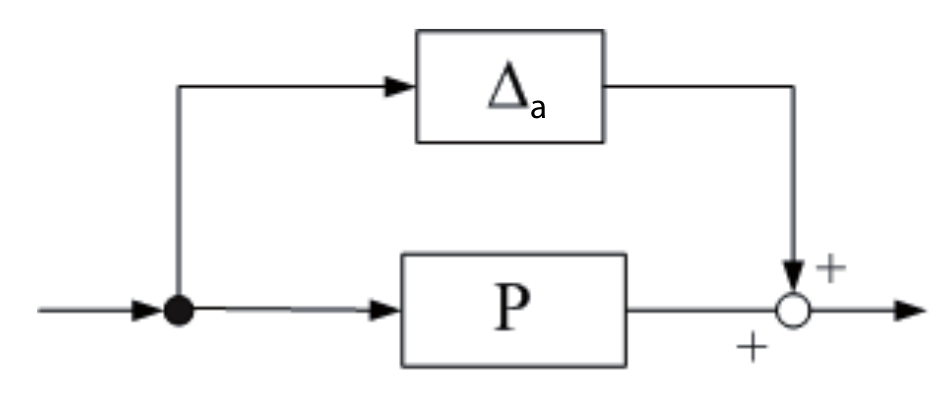
\includegraphics[width=4cm]{./bilder/rob_add.png}}
	\parbox{15cm}{
		$ \left \lVert \Delta_a \cdot \frac{-C}{1+P_0 C} \right\rVert_\infty < 1 $\\
		$ \Rightarrow \left \lVert \Delta_a \right\rVert_\infty < \frac{1}{\left \lVert \frac{C}{1+P_0 C} \right\rVert_\infty}$ da $\left \lVert AB \right\rVert < \left \lVert A \right\rVert \cdot \left \lVert b \right\rVert$\\
		$\Delta_a(s)=P(s) - P_0(s) \Rightarrow \left| \Delta_a(s) \right| < \left| W_{2a}(s)\tilde{\Delta} \right| $ suche $\left| W_{2a}(s) \right|  = \underset{par\in[]}{max} \left| \Delta_a(s) \right| $
		}
\end{tabular}		

\subsection{Multiplikative Unsicherheit}
	\parbox{5cm}{
	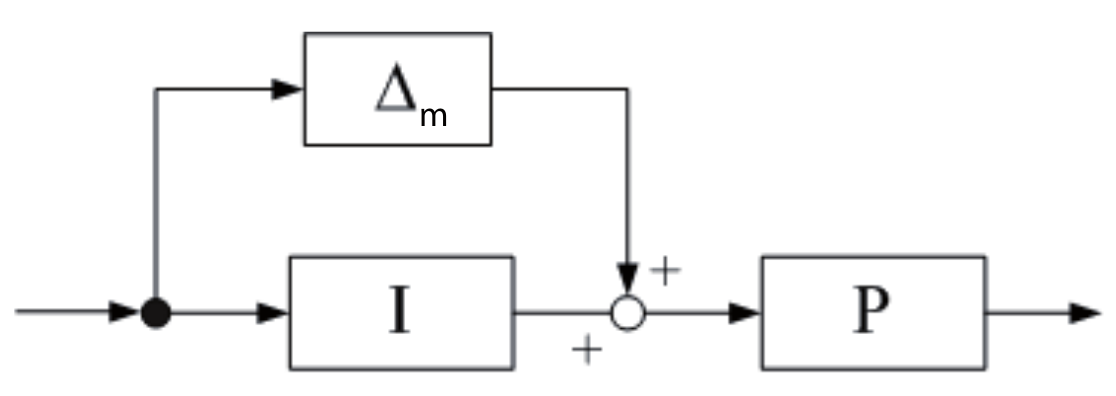
\includegraphics[width=4cm]{./bilder/rob_mult.png}}
	\parbox{15cm}{
		$ \left \lVert \Delta_m \cdot \frac{-P_0C}{1+P_0 C} \right\rVert_\infty < 1 $\\
		$ \Rightarrow \left \lVert \Delta_m \right\rVert_\infty < \frac{1}{\left \lVert \frac{P_0C}{1+P_0 C} \right\rVert_\infty}$ da $\left \lVert AB \right\rVert < \left \lVert A \right\rVert \cdot \left \lVert b \right\rVert$\\
		$\Delta_m(s)=\frac{P(s)}{P_0(s)} - 1 \Rightarrow \left| \Delta_m(s) \right| < \left| W_{2m}(s)\tilde{\Delta} \right| $ suche $\left| W_{2m}(s) \right|  = \underset{par\in[]}{max} \left| \Delta_m(s) \right| $
		}
		
\subsection{LFT}
	\parbox{6cm}{
	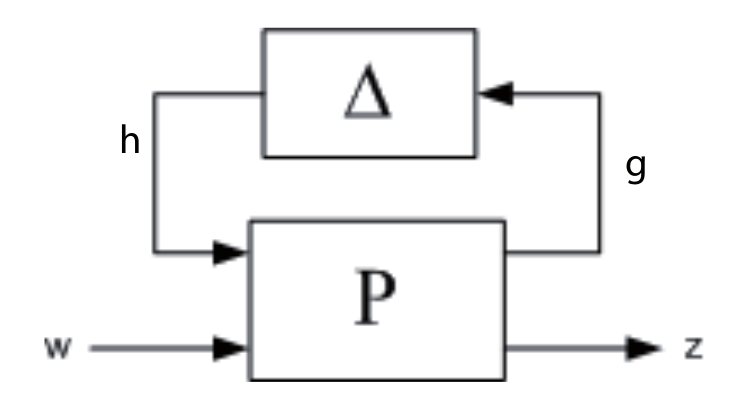
\includegraphics[width=4cm]{./bilder/rob_lft.png}\\
	$z=\left[ P_{22} + P_{21} \Delta(I-P_{11}\Delta)^{-1}P_{12}\right]w$}
	\parbox{4cm}{
		Additiv\\
		$P=\begin{bmatrix}
			0 && I \\
			I && P_0
		\end{bmatrix}$\\
		Multiplikativ\\
		$P=\begin{bmatrix}
			0 && P_0 \\
			I && P_0
		\end{bmatrix}$
		}
	\parbox{5cm}{
		Parameter $K=\bar{P}(1+P_\Delta\delta)$\\
		$P=\begin{bmatrix}
			0 && \bar{P} \\
			P_\Delta && \bar{P}
		\end{bmatrix}$\\
		Parameter $K=\frac{1}{\bar{P}(1+P_\Delta\delta)}$\\
		$P=\begin{bmatrix}
			-P_\Delta && \frac{1}{\bar{P}} \\
			-P_\Delta && \frac{1}{\bar{P}}
		\end{bmatrix}$
		}

\subsection{$H_\infty$}
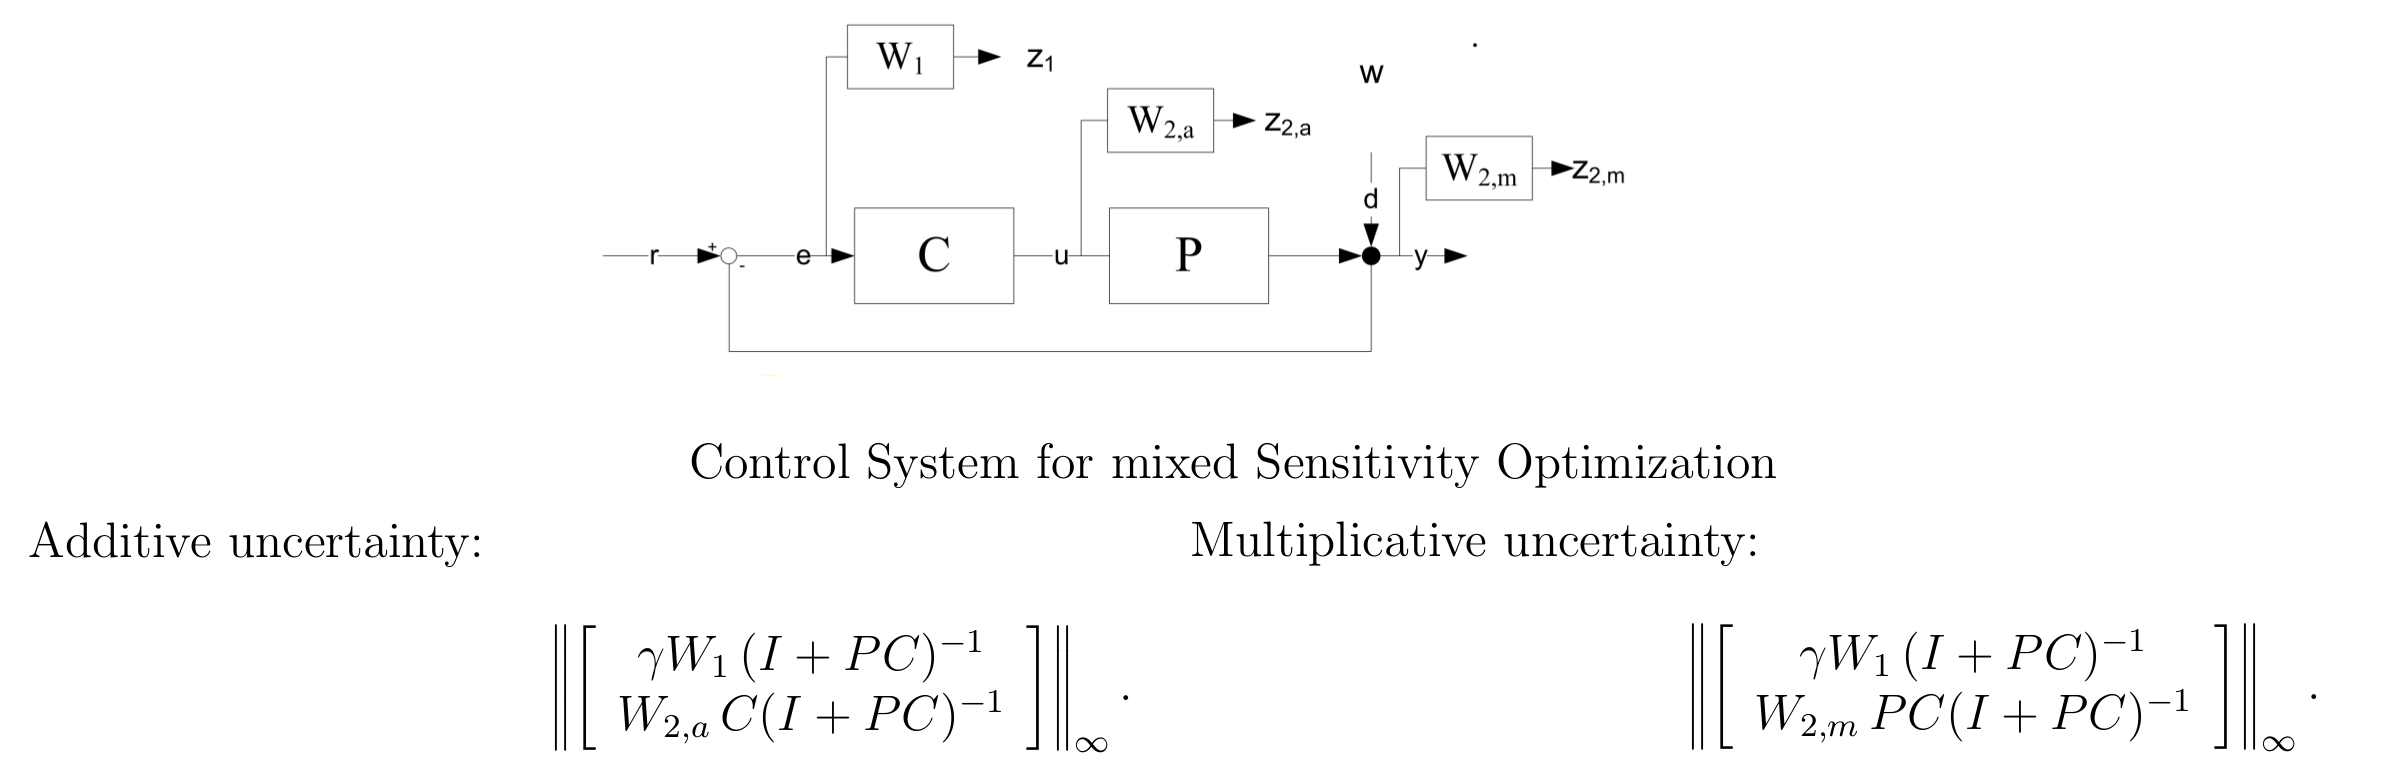
\includegraphics[width=15cm]{./bilder/rob_hinf.png}\\
    
    \newpage
    \section{Nichtlineare Regler}

\subsection{Lyapunov Redesign}

Nichtlineares System: $\dot{x} = f(x) + g(x) \cdot u$

Lyapunov-Funktion V(x) mit folgenden Eigenschaften:
\begin{enumerate}
	\item $V(0) = 0$ und $V(x) > 0 \quad \forall x \neq 0$
	\item $\dfrac{dV(x(t))}{dt}=\dfrac{dV(x)}{dx}\dfrac{dx(t)}{dt} \leq 0$ bedeutet Stabilität. $\dfrac{dV(x(t))}{dt} > 0$ bedeutet entweder Instabilität oder dass $V(x)$ keine geeignete Lyapunov-Funktion ist.
\end{enumerate}
    \newpage
    
    \section{Verschiedene Transformationen}
\begin{minipage}{13.5cm}
\subsection{Berechnung}
\tiny
\begin{tabular}{|l|l|l|}
\hline
  \textbf{Transformation}
  & \textbf{Vorwärts}
  & \textbf{Rückwärts} \\
\hline
  Fourier-Reihe
  & $c_k=\frac{1}{T}\int_0^T{f(t) e^{-jk\omega_1 t}dt}$
  & $f(t) = \sum\limits_{k = -\infty}^{\infty} c_k  e^{j k \omega_1 t}$ \\
\hline
  Fourier-Integral
  & $F(\omega) = \int\limits_{-\infty}^{\infty} f(t)e^{-j\omega t}dt$
  & $f(t) =  \frac{1}{2\pi}\int\limits_{-\infty}^{\infty}
    F(\omega)e^{j\omega t}d\omega$ \\
\hline
  Laplace-Transformation
  & $F(s)=\int\limits_0^\infty f(t)e^{-st}dt$
  & Polynomdivision $\Rightarrow$ Partialbruchzerlegung $\Rightarrow$ Tabelle!\\
\hline
  Diskrete Fouriertransformation
  & $F(k) = \sum\limits_{n=0}^{N-1} f(n) e^{-j 2 \pi \frac{n}{N} k}$
  & $f^*(k) = \frac{1}{N} DFT(F^* (k))$\\
\hline
  Z-Transformation ($z = e^{j s T}$)
  & $F(z) = \sum\limits_{n=0}^{\infty} f(n) z^{-n}$
  & Polynomdivision $\Rightarrow$ Partialbruchzerlegung $\Rightarrow$ Tabelle!\\
\hline
\end{tabular}
\normalsize
\end{minipage}
\begin{minipage}{5.5cm}
\subsection{Pol/Nullstellentransfo}
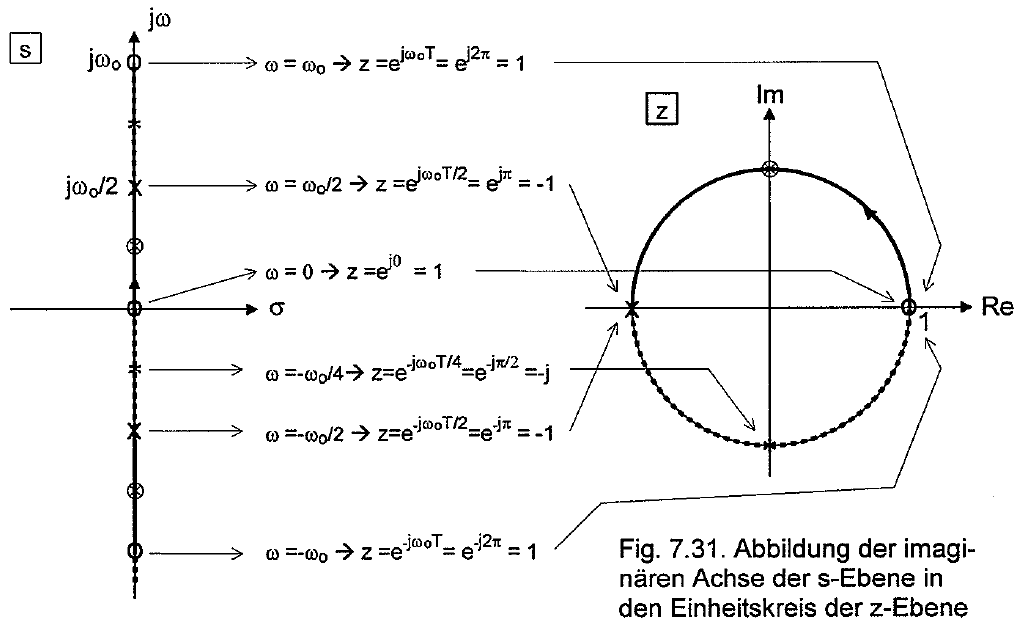
\includegraphics[width=5.5cm]{bilder/ImagAchse-Einheitskreis.png}
\end{minipage}

\section{Eigenschaften von Fourier- und Z-Transformation}
\tiny
\renewcommand{\arraystretch}{1.1}
\begin{tabular}{|p{3.2cm}||p{1.5cm}|p{1.8cm}||p{2.5cm}|p{2.5cm}||p{1.7cm}|p{3cm}|}
\hline
\textbf{Bezeichnung}
  & \multicolumn{2}{|c||}{\textbf{Zeitbereich}}
  & \multicolumn{2}{|c||}{\textbf{Kontinuierlicher Frequenzbereich}}
  & \multicolumn{2}{|c|}{\textbf{Diskreter Frequenzbereich}} \\
  & \textbf{kontinuierlich}
  & \textbf{diskret}
  & \textbf{Fourier-Integral}
  & \textbf{Laplace}
  & \textbf{Diskrete FT}
  & \textbf{Z-Transformation} \\
\hline
\hline
  Linearität
  & $\alpha\cdot f(t) + \beta\cdot g(t)$
  & $\alpha\cdot f(n) + \beta\cdot g(n)$
  & $\alpha\cdot F(\omega) + \beta\cdot G(\omega)$
  & $\alpha\cdot F(s) + \beta\cdot G(s)$
  & $\alpha\cdot F(n) + \beta\cdot G(n)$
  & $\alpha\cdot F(z) + \beta\cdot G(z)$\\
\hline
  "Ahnlichkeit / Zeitskalierung bzw. Spiegelung an Y-Achse
  &	$f(\alpha t)$
  & $f(-n)$
  & $\frac{1}{|\alpha|}F \left (\frac{\omega}{\alpha} \right)$
  & $\frac{1}{\alpha}F \left (\frac{s}{\alpha} \right )$
  & $F(-n)$
  & $F(z^{-1})$\\
\hline
  Dämpfung
  & -
  & $e^{dn} f(n)$
  & -
  & -
  & -
  & $F(z e^{d})$ \\
\hline
  Verschiebung im Zeitbereich
  & $f(t\pm t_0)$
  & $f(n \pm n_0)$
  & $e^{\pm j\omega t_0} F(\omega)$
  & $F(s)e^{\pm t_0 s}$
  & $e^{\pm j\frac{n}{N}2 \pi n_0} F(n)$
  & $z^{\pm n_0} F(z)$\\
\hline
  Verschiebung im Frequenzbereich
  & $f(t)e^{\mp\alpha t}$
  & $f(n) e^{\mp j \frac{n}{N} 2 \pi n_0}$
  & $F(\omega\pm \alpha)$
  & $F(s\pm\alpha)$
  & $F(n \pm n_0)$
  & $F(z \pm n_0)$\\
\hline
  Faltung im Zeitbereich
  &	$f(t) \ast g(t)$
  & $f(n) \ast g(n)$
  & $F(\omega) \cdot G(\omega)$
  & $F(s) \cdot G(s)$
  & $F(n) \cdot G(n)$
  & $F(z) \cdot G(z)$ \\
\hline
  Faltung im Frequenzbereich
  &	$f(t) \cdot g(t)$
  & $f(n) \cdot g(n)$
  & $\frac{1}{2\pi} F(\omega) \ast G(\omega)$
  & $\frac{1}{2\pi} F(s) \ast G(s)$
  & $\frac{1}{N} F(n) \ast G(n)$
  & $\frac{1}{N} F(z) \ast G(z)$\\
\hline
  Ableitungen im Zeitbereich bzw. Differenzenbildung
  & $\frac{\partial^n f(t)}{\partial t^n}$
  & $\Delta^k f(n)$
  & $(j\omega)^n F(\omega)$
  & $s^nF(s)-s^{n-1}f(0+)-s^{n-2}\frac{\partial f(0+)}{\partial t}-\ldots
 			-s^0\frac{\partial^{n-1} f(0+)}{\partial t^{n-1}}$
  &
  & $(1-z^{-1})^k F(z)$ \\
\hline
  Ableitung im Frequenzbereich
  & $(-t)^k\cdot f(t)$
  & $n f(n)$
  & $j^k \frac{-\partial^k F(\omega)}{\partial \omega^k}$
  & $\frac{\partial^k F(s)}{\partial s^k}$
  &
  & $-z \frac{\partial F(z)}{\partial z}$ \\
\hline
  Integration bzw. Summierung
  & $\int\limits_{-\infty}^t f(\tau)d\tau$
  & $\sum\limits_{n=0}^{k} f(n)$
  & $\frac{F(\omega)}{j\omega}+F(0)\pi\delta(\omega)$
  & $\frac{F(s)}{s}$
  &
  & $\frac{1}{1-z^{-1}} F(z)$ \\
\hline
  Anfangswert (Impulse)
  & $\lim\limits_{t\rightarrow 0} f(t)$
  & $f(0)$
  &
  & $\lim\limits_{s\rightarrow \infty} sF(s)$
  &
  & $\lim\limits_{z \rightarrow \infty} F(z)$ \\
\hline
  Endwert (Impulse)
  &	$\lim\limits_{t\rightarrow \infty} f(t)$
  & $\lim\limits_{n\rightarrow \infty} f(n)$
  &
  & $\lim\limits_{s\rightarrow 0} sF(s)$
  &
  & $\lim\limits_{z \rightarrow 1} ((1-z^{-1}) F(z))$\\
\hline
  Stabilität
  & -
  & -
  & -
  & Pole in LHE
  &
  & Pole innerhalb Einheitskreis \\
\hline
  Kausalität
  & -
  & -
  & A- \& Kausal
  & Nur Kausal
  &
  & $\lim\limits_{z \rightarrow \infty} z^{-1} F(z) = 0$ \\
\hline
\hline
  Spezial
  & \multicolumn{3}{l||}{
      Bessel-Theorem \qquad
      $\int\limits_{-\infty}^{\infty}f(t)g^{\ast}(t)dt =
         \frac{1}{2\pi}
         \int\limits_{-\infty}^{\infty}F(\omega)G^{\ast}(\omega)d\omega$}
  & \multicolumn{3}{|l|}{
      Parseval-Theorem \qquad
      $W = \int\limits_{-\infty}^{\infty}|f(t)|^2 dt = \frac{1}{2\pi}
      \int\limits_{-\infty}^{\infty}|F(\omega)|^2 d\omega$
    }\\
\hline
\end{tabular}
\renewcommand{\arraystretch}{1}\\
\normalsize

\begin{minipage}{11cm}
	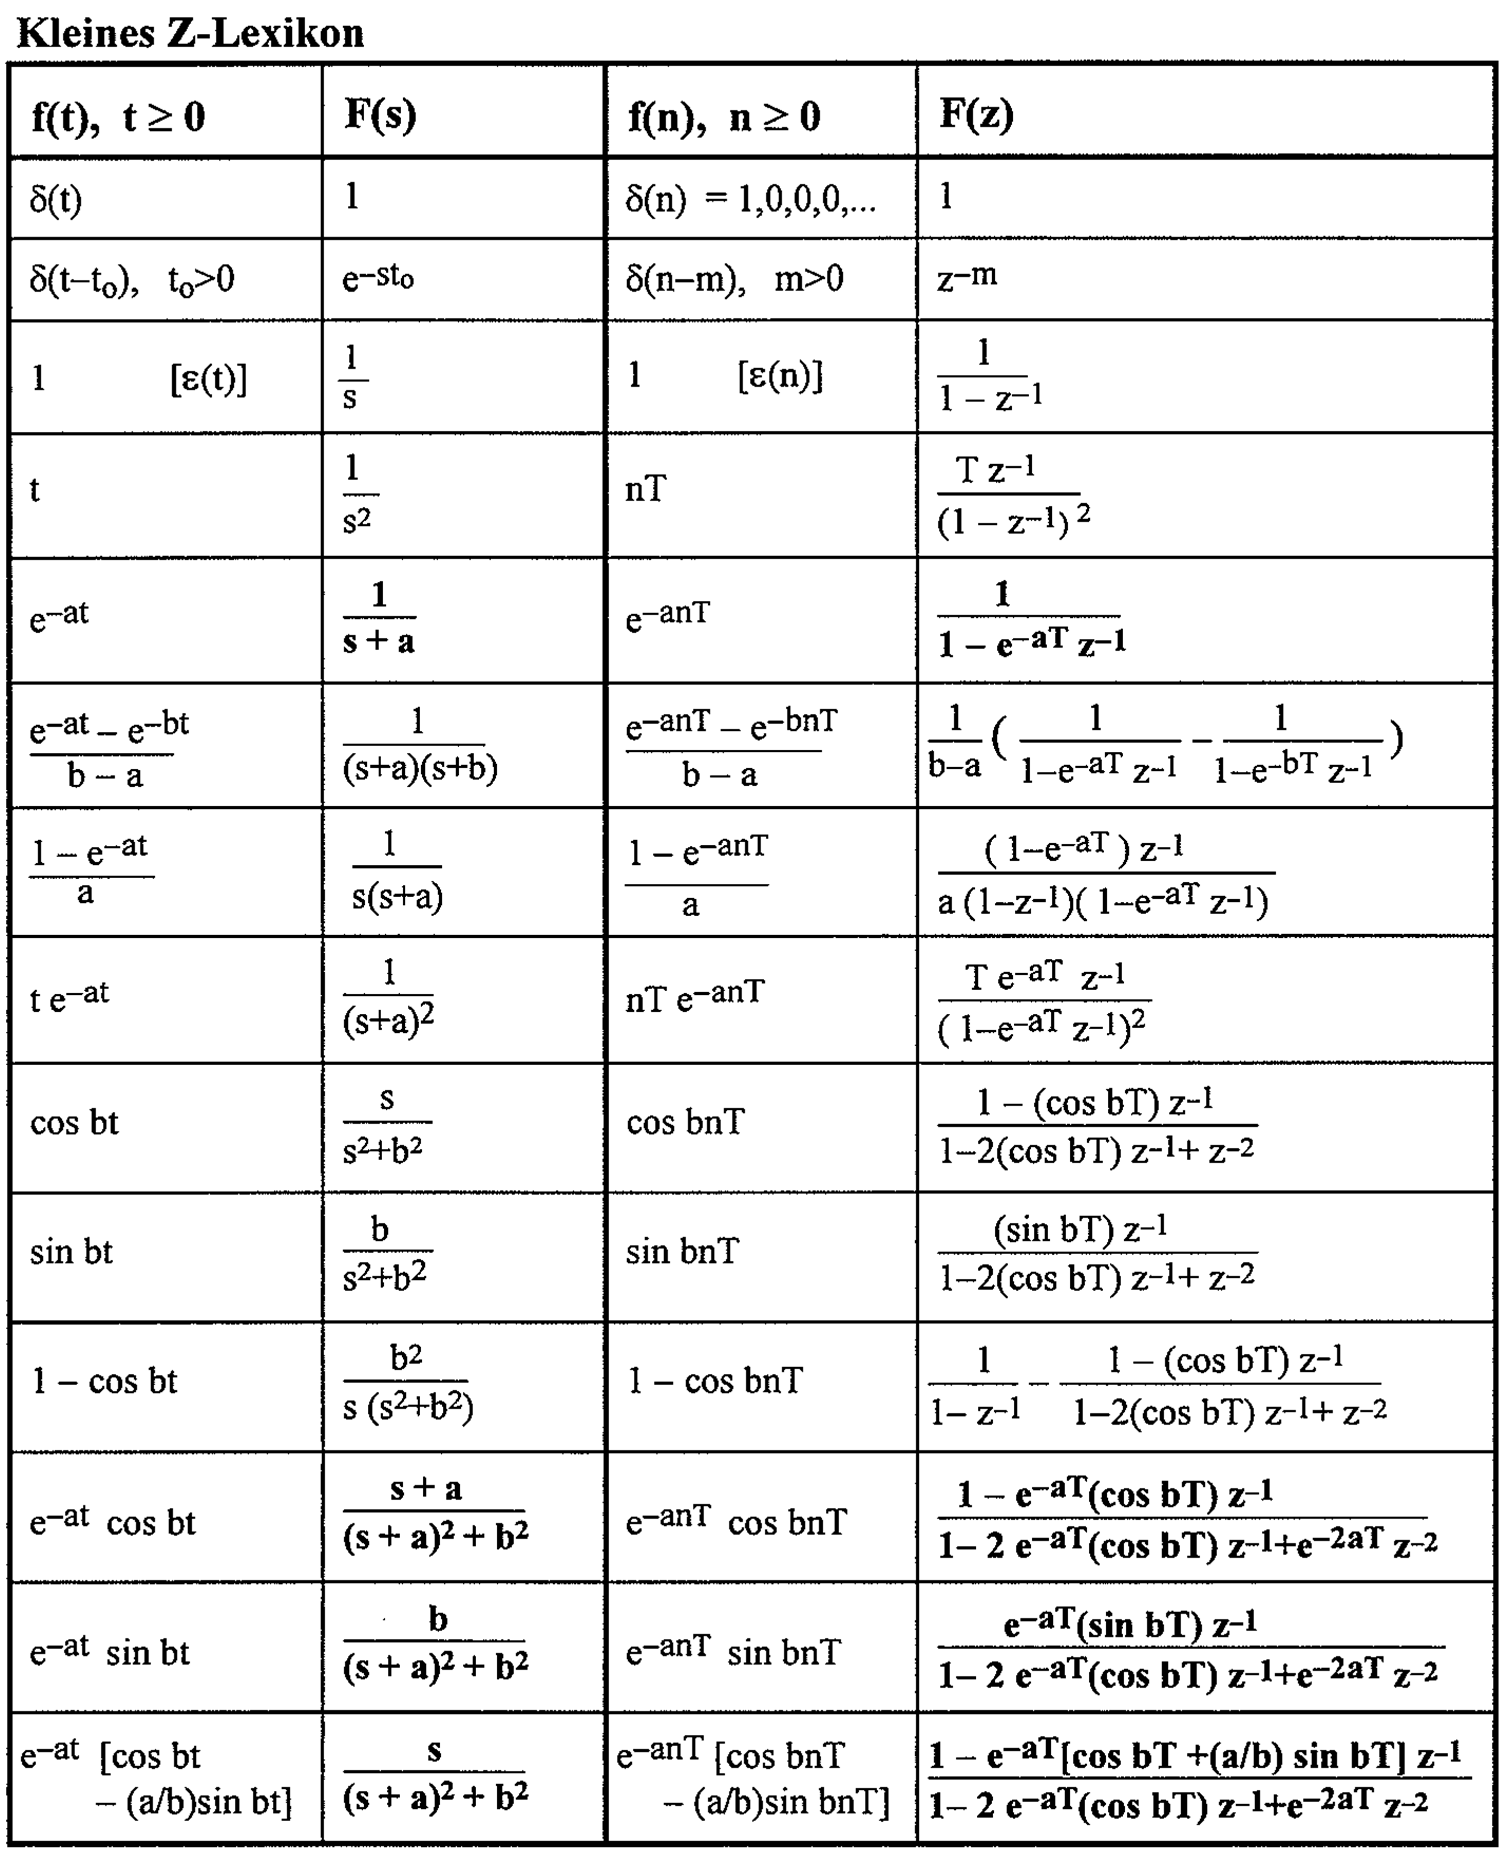
\includegraphics[height=11cm]{bilder/Z-Lexikon.png}
\end{minipage}
\begin{minipage}{8cm}
	Endwert Schrittantwort: $\lim\limits_{s\rightarrow 0} F(s)$ / $\lim\limits_{z \rightarrow 1} F(z)$\\
	$P_{ZOH}(z)=\frac{z-1}{z} Z_s \left\lbrace  \frac{P(s)}{s} \right\rbrace $\\
	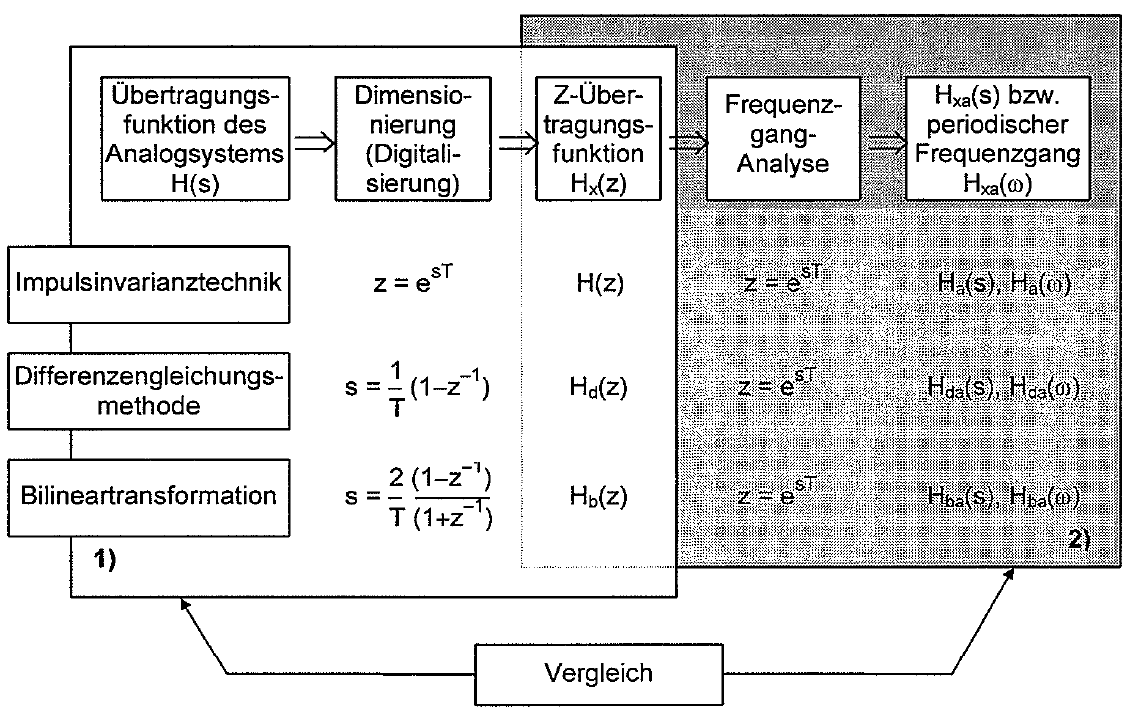
\includegraphics[width=8cm]{bilder/IIR-ArbeitsschritteundVarianten.png}\\
	PT1: $ F(s)=\frac{k}{1+Ts} \quad f(t) = k(1-e^{-\frac{t}{T}}) \quad \omega = \frac{1}{T}$\\
	PT2: $ F(s)=\frac{k}{1+2dTs + T^2s^2}$ \quad Pole bei: $\frac{d \pm \sqrt{d^2-1}}{T}$ \\
	\vspace*{0.5cm} bei $d \geq \frac{1}{\sqrt{2}}$ kein Überschwingen\\
	Feadback$\mp$: $G(s)=\frac{Z(s)}{N(s)} \rightarrow  \frac{Z(s)}{N(s) \pm Z(s)}$
\end{minipage}

    \newpage
    \section{Matrizenrechnung}
\scriptsize


\subsection{Determinante}

	\textbf{3x3 Matrix}
	$$ \det \begin{bmatrix} a_{11} & a_{12} & a_{13} \\ a_{21} & a_{22}& a_{23} \\
	a_{31} & a_{32} & a_{33} \end{bmatrix} \\ = a_{11} a_{22} a_{33} + a_{12}
	a_{23} a_{31} + a_{13} a_{21} a_{32} - a_{13} a_{22} a_{31} - a_{12} a_{21}
	a_{33} - a_{11} a_{23} a_{32}.  $$
	
	\textbf{Dreiecksmatrix} - Alle Elemente entweder ober- oder unterhalt der Hauptdiagonale $= 0$
	$$\det A =a_{11}\cdot a_{22}\dotsb a_{nn} \quad  \quad \text{Die Det. ist das Produkt
	der Hauptdiagonal-Einträge. Gilt somit auch für Diagonalmatritzen.} $$
	
	\textbf{Null $(|A| = 0)$} - Wenn $A$ eine (n,n)-Matrix ist, so wird $|A| = 0$ unter einer der
	folgenden Bedingungen:
	\begin{itemize}
    	\item Zwei Zeilen/Spalten sind linear abhängig (gleich oder ein Vielfaches der anderen).
    	\item Alle Elemente einer Zeile/Spalte sind Null. \\
  	\end{itemize} 
	
	\textbf{Allgemein:}
	$$A\epsilon M_n: \det A =    
	\begin{vmatrix}
    	a_{11} & a_{12}& \ldots & a_{1n}\\
    	a_{21}& &\ldots & \\
    	\ldots \\
    	a_{n1} & & \ldots & a_{nn}    			
    \end{vmatrix}=
	(-1)^{1+1}a_{11}D_{11} + (-1)^{1+2}a_{12}D_{12}+ \ldots +
	(-1)^{1+n}a_{1n}D_{1n}$$
	
	\subsubsection{Unterdeterminante}
	$$D_{11}=
	\begin{vmatrix}
    	a_{22} & \ldots & a_{2n}\\
    	\ldots\\
    	a_{n2}& \ldots & a_{nn}
    \end{vmatrix} 	\\
	D_{12}=
	\begin{vmatrix}
    	a_{21} & a_{23}& \ldots & a_{2n}\\
    	\ldots\\
    	a_{n1}& a_{n3}&\ldots & a_{nn}
    \end{vmatrix}$$\\
	$D_{ij}$ die (n-1)$ \times $(n-1)-Untermatrix von D ist, die durch Streichen der
	i-ten Zeile und j-ten Spalte entsteht.\\
	Diese Methode ist zu empfehlen, wenn die Matrix in einer Zeile oder Spalte
	bis auf eine Stelle nur Nullen aufweisst.
	Dies lässt sich meist mit dem Gausverfahren bewerkstelligen.
	
\subsection{Gaussverfahren}
	Durch Addition und Subtraktion einzelner Zeilen (auch von Vielfachen einer
	Zeile) werden einzelne Stellen auf Null gebracht. zB:\\
	$\begin{bmatrix}
    	a_{11} & a_{12}& \ldots & a_{1n}\\
    	a_{21}& &\ldots & \\
    	\ldots \\
    	a_{n1} & & \ldots & a_{nn}    			
    \end{bmatrix}=
	\begin{bmatrix}
    	a_{11} & a_{12}& \ldots & a_{1n}\\
    	k a_{21}-n a_{11}& ka_{22}-n a_{12}&\ldots & k a_{2n} - n a_{1n}\\
    	\ldots \\
    	a_{n1} & & \ldots & a_{nn}    			
    \end{bmatrix}$ \\
	Die n * erste Zeile wurde von der k * zweiten Zeile abgezogen ($a_{2.}= 
	k a_{2.}- n a_{1.}$)
	
\subsection{Inverse Matrix \small{(Existiert nur wenn Matrix regulär: $\det A \neq 0$)}}
\begin{minipage}{7cm}
	\textbf{2x2 Matrix:}    
	$$ A^{-1} = \begin{bmatrix} a & b \\ c & d \\ \end{bmatrix}^{-1} = \frac{1}{ad
	- bc} \begin{bmatrix} d & -b \\ -c & a \\ \end{bmatrix} $$
\end{minipage}
\begin{minipage}{11cm}
	\textbf{3x3 Matrix:}
  $$  A^{-1} = \begin{bmatrix} a & b & c\\ d & e & f \\ g & h & i \\ \end{bmatrix}^{-1} =
  \frac{1}{\det(A)} \begin{bmatrix} ei - fh & ch - bi & bf - ce \\ fg - di & ai
  - cg & cd - af \\ dh - eg & bg - ah & ae - bd \end{bmatrix} $$
\end{minipage}\\

\textbf{Diagonalmatrix} (Alle Elemente ausserhalb der Hauptdiagonale $= 0$, Elemente auf
Hauptdiagonale sind Eigenwerte $\lambda_i$): \\ 
Alle Elemete elementweise invertieren - Kehrwert. $\quad \Rightarrow \quad $\textit{Gilt nur wenn
alle Elemente auf der Hauptdiagonale $\neq 0$ sind.}\\

\textbf{Allgemein:}\\
	$A^{-1}= \begin{bmatrix}
    	a_{11} & a_{12}& \ldots & a_{1n}\\
    	a_{21}& &\ldots & \\
    	\ldots \\
    	a_{n1} & & \ldots & a_{nn}    			
    \end{bmatrix}^{-1}$
	\begin{enumerate}
		\item $A^T$ bestimmen (Zeilen und Spalten vertauschen) $A^{T}= \begin{bmatrix}
    	a_{11} & a_{21}& \ldots & a_{n1}\\
    	a_{12}& &\ldots & \\
    	\ldots \\
    	a_{1n} & & \ldots & a_{nn}    			
    \end{bmatrix}$	
		\item Bei $A^T$ jedes Element $a_{ij}$ durch Unterdet. $D_{ij}$ mit
		richtigem Vorzeichen ersetzen $A^*=	\begin{bmatrix}
			(-1)^{1+1}D_{11} &  \ldots	& (-1)^{1+n} D_{1n}\\
			\ldots\\
			(-1)^{n+1} D_{n1}& \ldots  & (-1)^{n+n} D_{nn}
		\end{bmatrix}$
		\item $A^{-1} = \frac{A^*}{\det A}$ 
    \end{enumerate}
 
 \subsection{Diagonalisierung}
 	\begin{enumerate}
       \item Eigenwerte $\lambda$ auschrechnen: $\det (A - I_n \lambda)=0$
       \item Eigenvektoren $\vec{v}$ bilden: $(A- \lambda I_n)\vec{v}=0$
       \item Transformationsmatrix: $T= [\vec{v_1} \ldots \vec{v_n}]$
       \item $T^{-1}$ berechnen (Achtung ist A symmetrisch, dh. $A^T=A$ und
       oder alle EV senktrecht zueinander, dann $T^{-1}=T^T$)
       \item $D=\begin{bmatrix}
                	\lambda_1 &0 &0\\
                	0& \lambda_2 &0\\
                	0& 0& \lambda_3
                \end{bmatrix}$
		\item $A^n = T D^n T^{-1}$

     \end{enumerate}

    \newpage
\end{document}
